\documentclass[12pt,twocolumn]{article}
\usepackage[margin=1.5cm]{geometry}
\usepackage{amsmath}
\usepackage{graphicx}
\usepackage{hyperref}
\usepackage{sectsty}
\title{Midterm 2}
\author{Prof. Jordan C. Hanson}
\sectionfont{\fontsize{12}{15}\selectfont}

\begin{document}
\maketitle
\small

\section{Unit 4: Magnetism II}

\begin{figure}
\centering
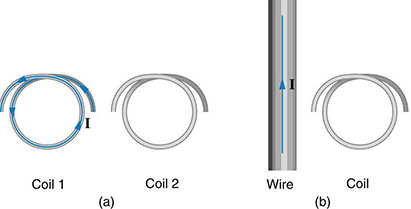
\includegraphics[width=0.4\textwidth]{B-flux.jpeg}
\caption{\label{fig:B-flux} \small (a) A current $I$ flows in the left coil, in the same plane as the right coil. (b) A wire with current $I$ flows in the same plane as the coil.}
\end{figure}
\begin{figure}
\centering
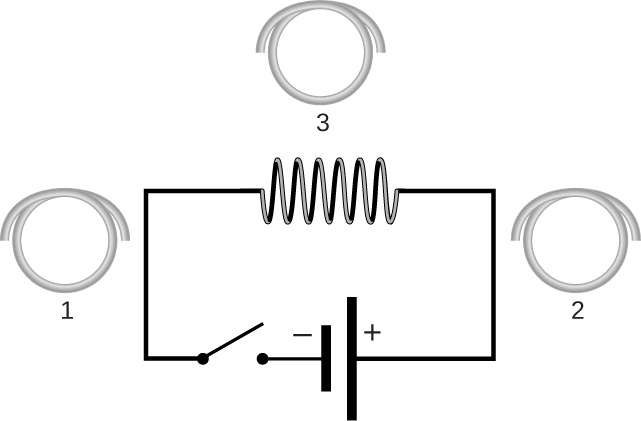
\includegraphics[width=0.4\textwidth]{awesome.jpeg}
\caption{\label{fig:B-flux2} \small A battery provides and emf to a simple circuit with a solenoid, surrounded by three wire loops \textit{in the plane of the circuit}.}
\end{figure}

\noindent
\begin{enumerate}
\item Consider Fig. \ref{fig:B-flux}a.  (a) What is the direction of the current induced in coil 2 if the current in coil 1 increases? If it decreases?  Consider Fig. \ref{fig:B-flux}b.  (b) What is the direction of the current induced in the coil if the current in the wire increases?  If it decreases? \\ \vspace{3cm}
\item Consider Fig. \ref{fig:B-flux2}.  (a) What is the direction of the current induced in coil 1 when the switch is closed?  If it is left closed for a long time?  When it is opened?  (b) Repeat exercise (a) for coil 2.  (c) Repeat exercise (a) for coil 3. \\ \vspace{3cm}
\item Verify that the units of $\Delta\phi/\Delta t$ are Volts. \\ \vspace{3cm}
\item (a) An MRI technician moves his hand from a region of very low magnetic field strength into an MRI scanner's 2.00 T field with his fingers pointing in the direction of the field. Find the average emf induced in his wedding ring, given its diameter is 2.20 cm and assuming it takes 0.250 s to move it into the field. (b) What current is induced in the ring if its resistance is 0.0100 $\Omega$?  (c) Calculate the average power dissipated in the ring. \\ \vspace{4cm}
\clearpage
\item Prove that when $B$, $l$, and $v$ are not mutually perpendicular, motional emf is given by $emf = Blv\sin\theta$. If $v$ is perpendicular to $B$, then $\theta$ is the angle between $l$ and $B$. If $l$ is perpendicular to $B$, then $\theta$ is the angle between $v$ and $B$. \textit{Hint: it is helpful to draw a diagram to define the angle $\theta$.}\\ \vspace{6cm}
\item (a) A bicycle generator rotates at 1875 rad/s, producing an 18.0 V peak emf. It has a 1.00 by 3.00 cm rectangular coil in a 0.640 T field. How many turns are in the coil? (b) What is the period of the AC output of the generator?  \\ \vspace{3cm}
\item An American traveler in New Zealand carries a transformer to convert New Zealand's standard 240 V to 120 V so that she can use some small appliances on her trip. (a) What is the ratio of turns in the primary and secondary coils of her transformer? (b) What is the ratio of input to output current? (c) How could a New Zealander traveling in the United States use this same transformer to power her 240 V appliances from 120 V? \\ \vspace{3cm}
\item Consider Fig. \ref{fig:B-flux2}.  Suppose coil 3 ($N=1$ turn) is rotated 90 degrees such that its normal direction is aligned with the normal direction of the solenoid ($N=6$ turns).  The system is now acting as a \textbf{transformer}.  Suppose the emf in the solenoid is given by $V(t) = V_0 \sin(\omega t)$. (a) Draw a graph of $V(t)$, with the x-axis and y-axis units labeled.  (b) Add the induced emf in coil 3 to your graph, assuming the magnetic flux in coil 3 is rendered identical to that in the solenoid with an iron core.  (c) If $V_0 = 120$ V, and $\omega = (240\pi)$ Hz, when does $V(t) = 0$? When does the induced emf in coil 3 equal zero? \\ \vspace{4cm}
\item Camera flashes charge a capacitor to high voltage by switching the current through an inductor on and off rapidly. In what time must the 0.100 A current through a 2.00 mH inductor be switched on or off to induce a 500 V emf? \\ \vspace{1cm}
\item A large research solenoid has an inductance of 25.0 H. (a) What induced emf opposes shutting it off when 100 A of current through it is switched off in 80.0 ms? (b) How much energy is stored in the inductor at full current? (c) At what rate in watts must energy be dissipated to switch the current off in 80.0 ms? (d) Considering exercise (c), is it surprising that shutting it down this quickly is difficult? (d) Design a solenoid that has an inductance of 25.0 H by choosing the number of turns $N$, the cross-sectional area $A$, and the number of turns $l$. \\ \vspace{4cm}
\item Your RL circuit has a characteristic time constant of 20.0 ns, and a resistance of 5.00 M$\Omega$. (a) What is the inductance of the circuit? (b) What resistance would give you a 1.00 ns time constant, perhaps needed for quick response in an oscilloscope? (c) Suppose you design for a 1.00 ns time constant.  What percentage of the final current $I_0$ flows 3.0 ns after the circuit is closed? (d) What is the reactance of the inductor at 10 kHz? \\ \vspace{2cm}
\item An inductor designed to filter high-frequency noise from power supplied to a personal computer is placed in series with the computer. What minimum inductance should it have to produce a 2.00 k$\Omega$ reactance for 15.0 kHz noise? (b) What is its reactance at 60.0 Hz? \\ \vspace{1.5cm}
\item Consider Fig. \ref{fig:RC}.  Assume the bottom wire is grounded at 0V.  (a) Considering the capacitor reactance, describe why the circuit acts as a \textit{low-pass filter.}  That is, AC signals at $v_{\rm in}$ with \textit{high} frequencies produce very small amplitudes at $v_{\rm out}$. (b) Using Kirchhoff's loop rule on the left side of the circuit, write an equation that describes changes in potential.  (c) Repeat exercise (b) for the right loop.  (d) Solve parts (b) and (c) for $v_{\rm in}$ and $v_{\rm out}$, respectively, and calculate $v_{\rm out}/v_{\rm in}$ in terms of $R$ and $C$.  (e) What is the value of $v_{\rm out}/v_{\rm in}$ for $f = 100(2\pi R C)^{-1}$? For $f = 0.1(2\pi R C)^{-1}$? \\ \vspace{6cm}
\item (a) What are the resonance frequency, $f_0$, and resonance width, $\Delta f/f_0$, of an RLC circuit with $R = 0.1$ k$\Omega$, $C = 1$ $\mu$F, and $L = 1$ $\mu$H? (b) What is the reactance of this circuit at $f = 0.1f_0$ and $f = 10f_0$? \\ \vspace{3cm}
\item For an RLC circuit with that values of $R$, $L$, and $C$ from the previous problem, and AC source voltage characterized by $V_{\rm rms} = 120$ V, (a) what is $I_{\rm rms}$ at $10 f_0$ and $0.1 f_0$? (b) What is $P_{\rm rms}$ at these frequencies? \textit{Hint: calculate the phase angle between resistance and reactance.} \\ \vspace{4cm}
\item Suppose we are using an LC resonator and diode combination to create an AM radio signal.  If the resonance frequency of our resonator is 1.4 MHz, and our audio signal is at 10 kHz, (a) what three frequencies should be present in our AM radio spectrum?  (b) Suppose our receiver was receiving only the carrier frequency, but not either modulation peak.  Should we gradually increase or gradually decrease the resistance of the receiver circuit?  \\ \vspace{2cm}
\end{enumerate}

\section{Unit 5: Waves, Optics, Medical Physics}

\noindent
\begin{enumerate}
\item What 
\end{enumerate}

\begin{figure}[hb]
\centering
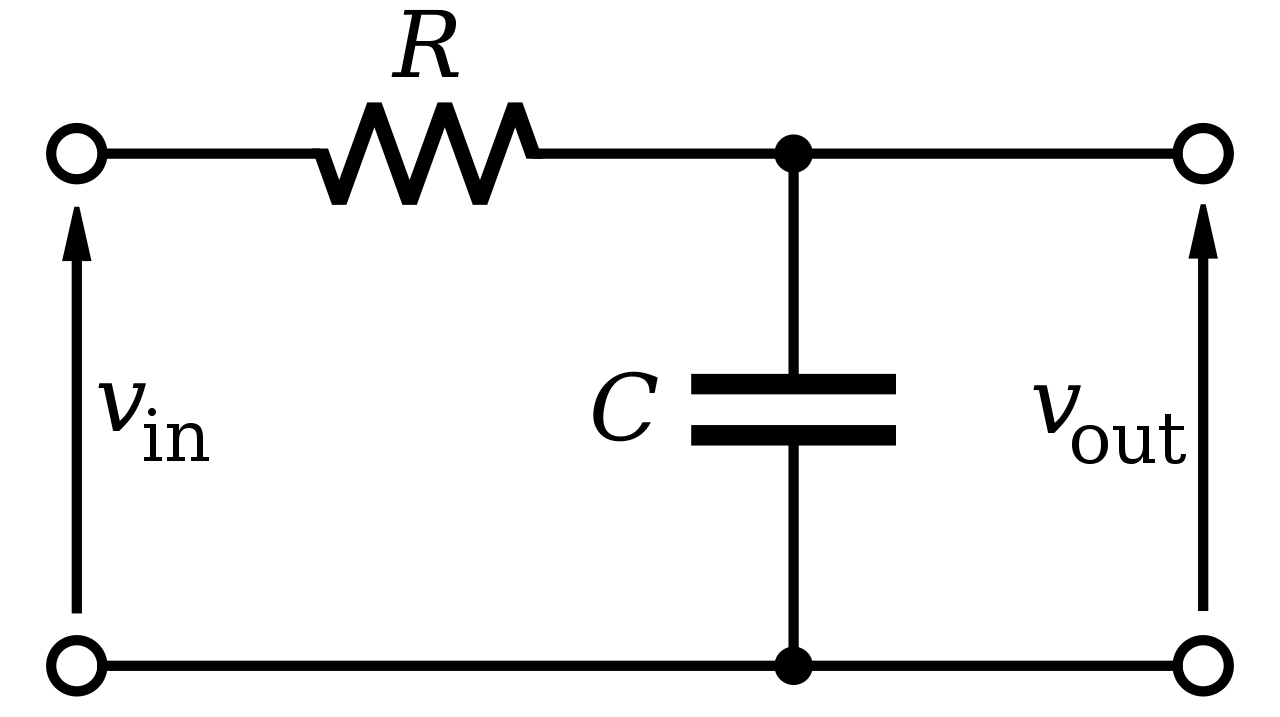
\includegraphics[width=0.3\textwidth]{low-pass.png}
\caption{\label{fig:RC} \small This is a series RC circuit, acting as a low-pass filter.}
\end{figure}

\end{document}